\documentclass[12pt]{article}

\usepackage{geometry}
\geometry{a4paper, left=1in, right=1in, top=1in, bottom=1in}
\usepackage{amsmath}
\usepackage{amsmath,amsfonts,amssymb}
\usepackage{graphicx,subcaption,lipsum}
\usepackage{enumitem}
\usepackage{titlesec}
\usepackage{fancyhdr}
\usepackage{hyperref}
\usepackage{floatrow}
\usepackage{geometry}
\usepackage{fancyhdr}
\usepackage{empheq}
\usepackage[svgnames]{xcolor}
\usepackage{xpatch}
\usepackage{float}

\makeatletter
\newcommand{\colorboxed}[1]{\fcolorbox{Black}{White}{\m@th$\displaystyle#1$}}
\xpatchcmd{\@Aboxed}{\boxed}{\colorboxed}{}{}
\makeatother

\title{{\bf CS663 Assignment 3}}
\author{Saksham Rathi, Kavya Gupta, Shravan Srinivasa Raghavan}
\date{September 2024}
\begin{document}
\maketitle
\clearpage

\section*{Question 1}

\textbf{Note:} All the Fourier Transform and Frequency Response figures are shown in logarithm absolute format.

\subsection*{Original Image}
\begin{figure}[H]
    \begin{subfigure}{.45\textwidth}
    \centering
      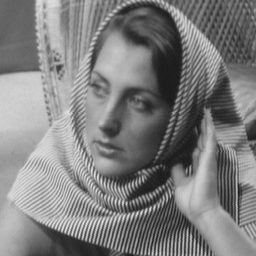
\includegraphics[width=1\linewidth]{../images/barbara256.png}
      \caption{Original Image}
    \end{subfigure}
    \begin{subfigure}{.5\textwidth}
    \centering
      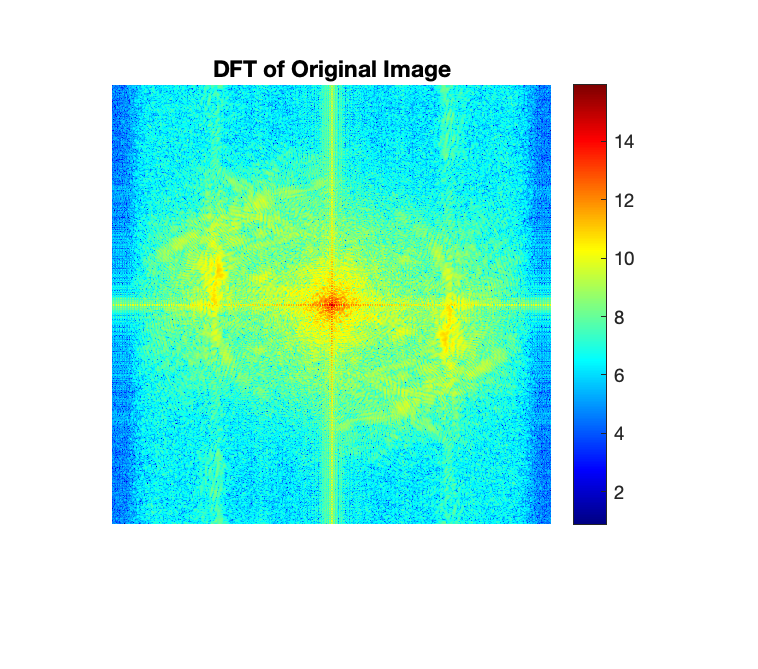
\includegraphics[width=1\linewidth]{../images/barbara_original_DFT.png}
      \caption{Fourier Transform of Original Image}
    \end{subfigure}
\end{figure}

\subsection*{Ideal Low Pass Filter}

\subsubsection*{Cutoff Frequency = 40}
\begin{figure}[H]
    \begin{subfigure}{.45\textwidth}
    \centering
      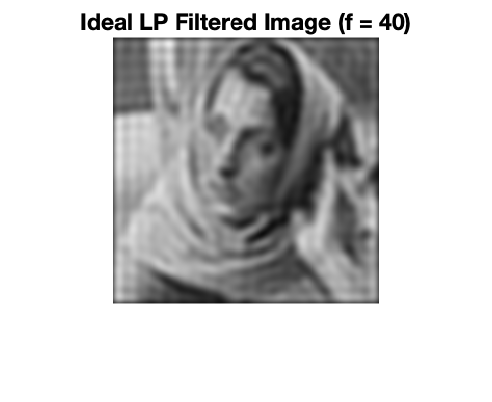
\includegraphics[width=1\linewidth]{../images/barbara_ideal_LPF_40.png}
      \caption{Filtered Image}
    \end{subfigure}
    \begin{subfigure}{.5\textwidth}
    \centering
      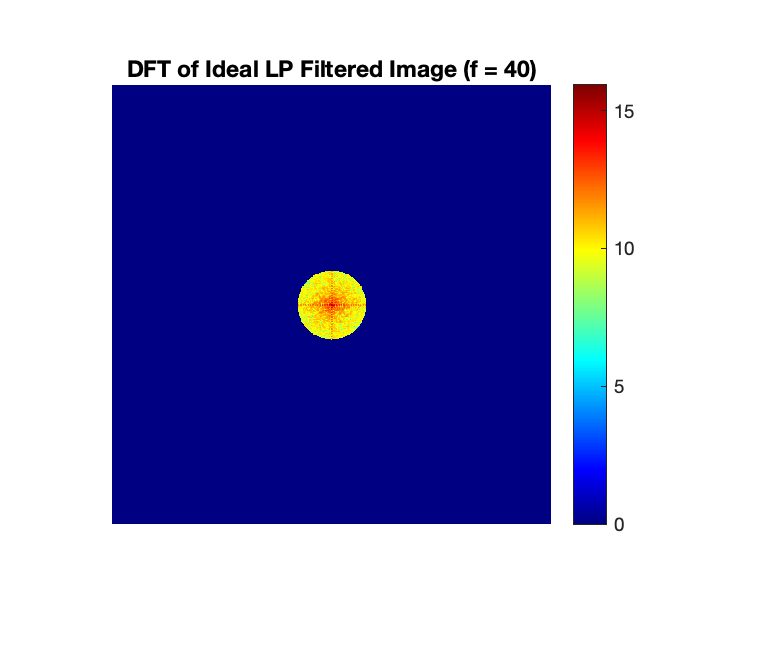
\includegraphics[width=1\linewidth]{../images/barbara_DFT_ideal_LPF_40.png}
      \caption{Fourier Transform of Filtered Image}
    \end{subfigure}
\end{figure}

\begin{figure}[H]
    \centering
    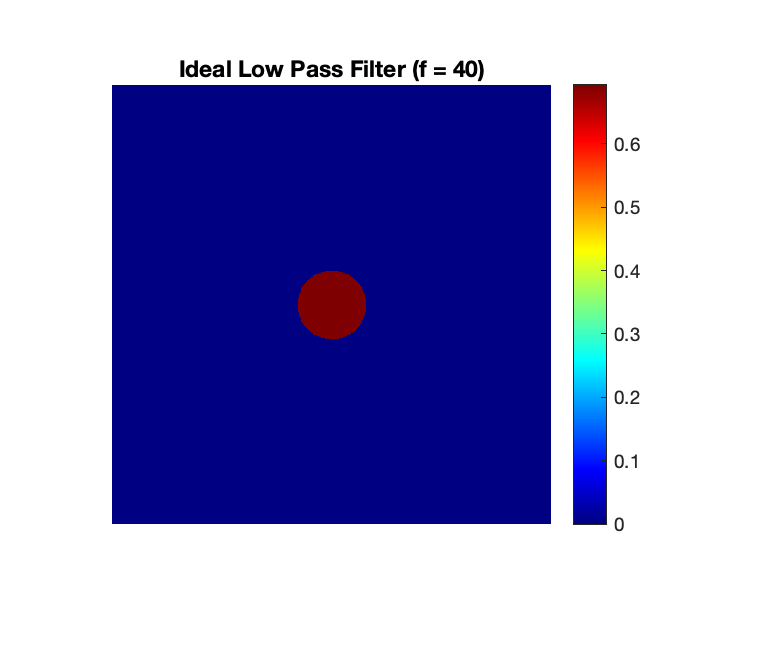
\includegraphics{../images/ideal_LPF_40.png}
    \caption{Frequency Response of Filter}
\end{figure}

\subsubsection*{Cutoff Frequency = 80}
\begin{figure}[H]
    \begin{subfigure}{.45\textwidth}
    \centering
      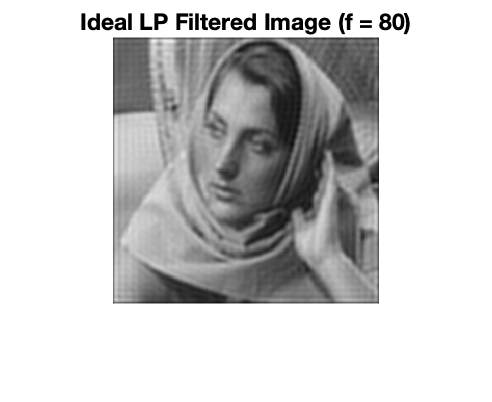
\includegraphics[width=1\linewidth]{../images/barbara_ideal_LPF_80.png}
      \caption{Filtered Image}
    \end{subfigure}
    \begin{subfigure}{.5\textwidth}
    \centering
      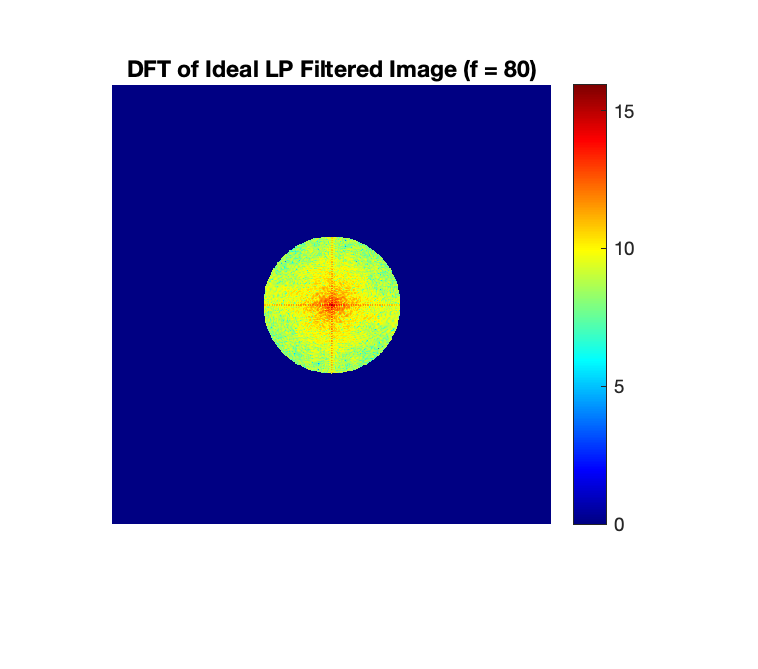
\includegraphics[width=1\linewidth]{../images/barbara_DFT_ideal_LPF_80.png}
      \caption{Fourier Transform of Filtered Image}
    \end{subfigure}
\end{figure}

\begin{figure}[H]
    \centering
    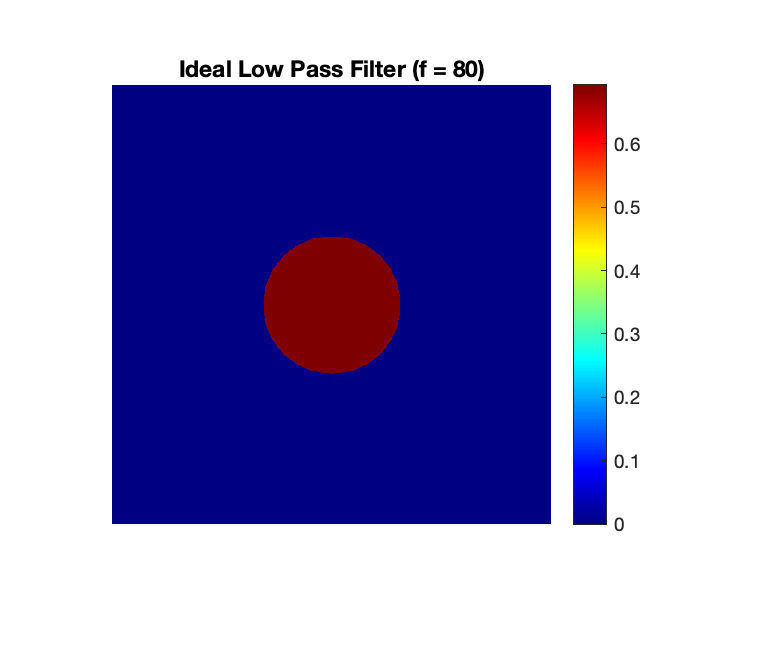
\includegraphics{../images/ideal_LPF_80.png}
    \caption{Frequency Response of Filter}
\end{figure}

\subsection*{Gaussian Low Pass Filter}

\subsubsection*{Sigma = 40}
\begin{figure}[H]
    \begin{subfigure}{.45\textwidth}
    \centering
      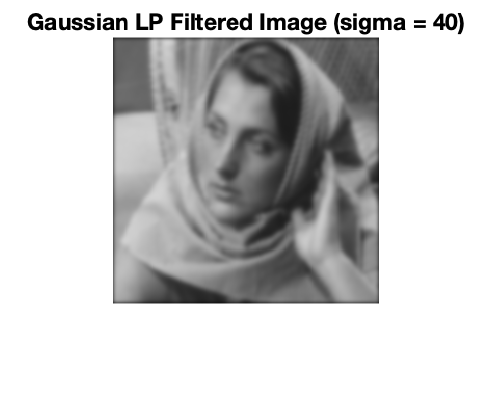
\includegraphics[width=1\linewidth]{../images/barbara_gaussian_LPF_40.png}
      \caption{Filtered Image}
    \end{subfigure}
    \begin{subfigure}{.5\textwidth}
    \centering
      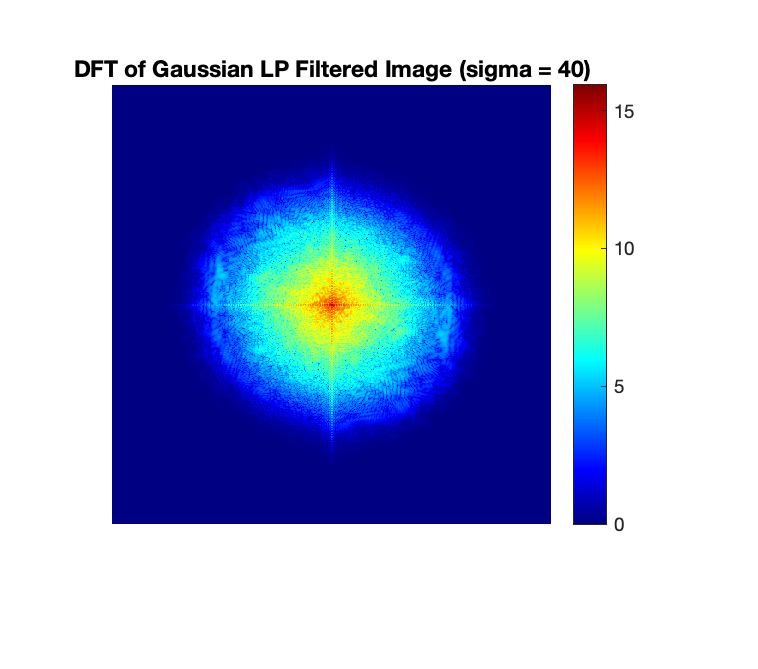
\includegraphics[width=1\linewidth]{../images/barbara_DFT_gaussian_LPF_40.png}
      \caption{Fourier Transform of Filtered Image}
    \end{subfigure}
\end{figure}

\begin{figure}[H]
    \centering
    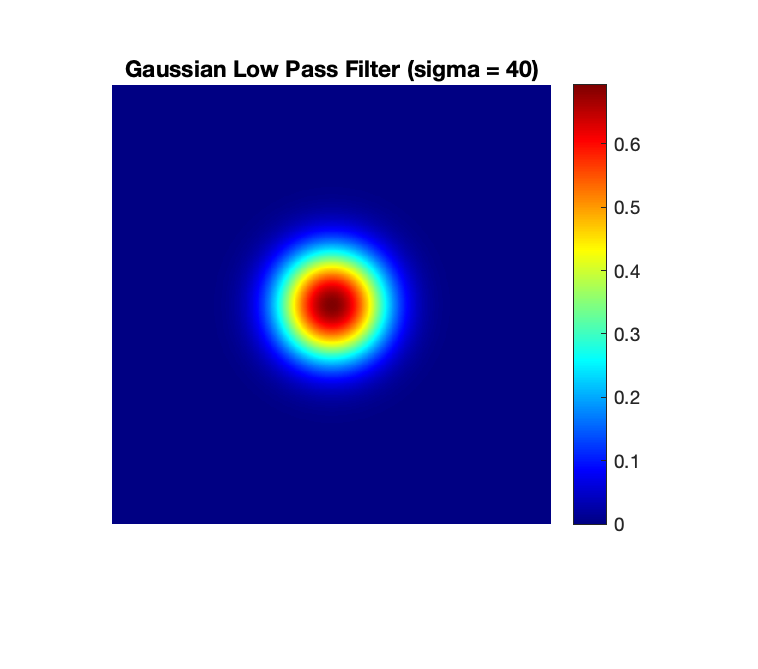
\includegraphics{../images/gaussian_LPF_40.png}
    \caption{Frequency Response of Filter}
\end{figure}

\subsubsection*{Sigma = 80}
\begin{figure}[H]
    \begin{subfigure}{.45\textwidth}
    \centering
      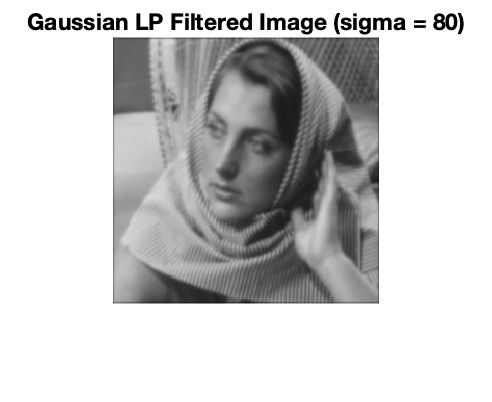
\includegraphics[width=1\linewidth]{../images/barbara_gaussian_LPF_80.png}
      \caption{Filtered Image}
    \end{subfigure}
    \begin{subfigure}{.5\textwidth}
    \centering
      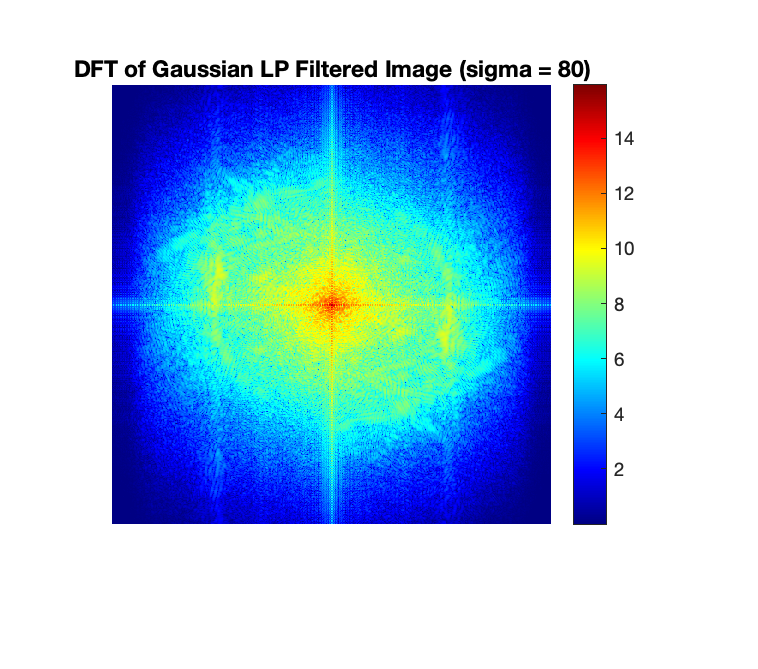
\includegraphics[width=1\linewidth]{../images/barbara_DFT_gaussian_LPF_80.png}
      \caption{Fourier Transform of Filtered Image}
    \end{subfigure}
\end{figure}

\begin{figure}[H]
    \centering
    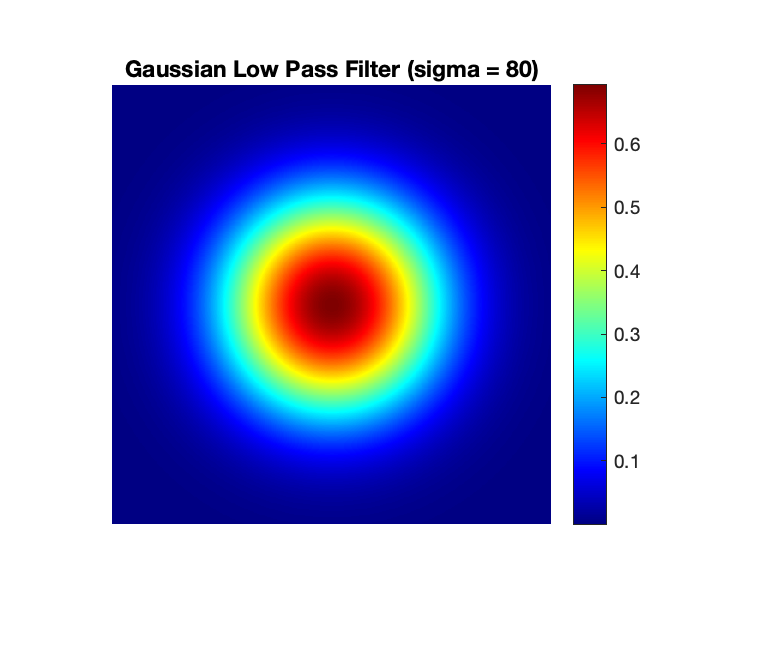
\includegraphics{../images/gaussian_LPF_80.png}
    \caption{Frequency Response of Filter}
\end{figure}

\subsection*{Observations}

\begin{itemize}
    \item From the obtained results we can easily see that as the cut-off frequency (for ideal low pass
    filter) / sigma (for Gaussian low pass filter) is increased, the higher frequency components
    which correspond to finer details in the image start becoming clearly visible.
    \item Also we can see that for ideal low pass filter there is a presence of \textbf{ringing artifacts} that appear
    as spurious signals near sharp transitions in the images. These ringing artifacts are quite
    undesirable and are a result of the complete elimination of high frequencies higher than the
    cut-off frequency by the ideal low pass filter.
    \item When a Gaussian low pass filter is used these ringing artifacts are absent.\ This is because the
    Gaussian low pass filter does not completely eliminate the higher frequencies and rather weakens
    them.
    \item In the Filtered Fourier Transform, we can see that Ideal Low Pass Filter creates sharp boundaries (beyond some distance from the centre), whereas the Gaussian doesn't have one, as we move away from the centre, the Fourier gradually fades away.
\end{itemize}
\end{document}